% To build a PDF version :
% $ xelatex leaflet-piwigo-fr.tex
\documentclass[12pt,nofoldmark,notumble]{leaflet}
\usepackage[utf8]{inputenc}
\usepackage[T1]{fontenc}
\usepackage[french]{babel}
\usepackage{libertine}
\renewcommand{\familydefault}{\sfdefault}
\usepackage{microtype}
\usepackage{menukeys}
\usepackage{graphicx}
\usepackage{fontawesome}
\usepackage{courier}
\usepackage{titlesec}
\usepackage{color}
\usepackage{verbatim}
\usepackage{enumitem}

\usepackage{tabularx}
\usepackage{array}
\usepackage{multirow}

\newcolumntype{o}{>{\hsize=.05\hsize}X}
\newcolumntype{s}{>{\hsize=.2\hsize}X}

\usepackage[para]{footmisc}

\setitemize{label=--}
\setenumerate[1]{label=\textcircled{\scriptsize\arabic*},
  font=\sffamily}
\pagenumbering{gobble}
\CutLine*{3}
\titlespacing\section{0pt}{12pt plus 4pt minus 2pt}{0pt plus 2pt minus 2pt}

% Colors
\definecolor{orange}{RGB}{255,119,0}

\titleformat{\section}
{\color{orange}\normalfont\normalsize\bfseries}
{\color{orange}\thesection}{1em}{}

\begin{document}
% \title{Communication}
% \date{}
% \author{\textsc{Galerie photo}}

% \maketitle

\begin{center}
  
\includegraphics[height=5cm,keepaspectratio]{logo.png}%
\end{center}

\section{Öffnungszeitun:}
\begin{tabular}{lp{8.3cm}}
  Montag & \emph{von} 11:30 \emph{bis} 21:30 \\
  Dienstag & Ruhetag \\
  Mittwoch & \emph{von} 11:30 \emph{bis} 21:30 \\
  Donnerstag & \emph{von} 11:30 \emph{bis} 21:30 \\
  Freitag & \emph{von} 11:30 \emph{bis} 21:30 \\
  Samstag & \emph{von} 11:30 \emph{bis} 21:30 \\
  Sonntag & \emph{von} 13:30 \emph{bis} 21:30
\end{tabular}

\section{Mindestbestellwert:}
\begin{tabular}{lp{8.3cm}}
  Ort & Preis \\
  % \cmidrule(r){1-2}
  Gröbenzell & ab €10,- \\
  Puchheim & ab €10,- \\
  Andere Orte & ab €16,-
\end{tabular}

\section{Telefonnummer:}
08143 4101910

\section{Anschrift:}
Am Zillerhof 5\\
Gröbenzell

\begin{center}
  
\includegraphics[height=1cm,keepaspectratio]{asiaXpress_homepage_head.png}%
\end{center}

\clearpage

\section{Suppen}

\begin{tabularx}{1.0\textwidth} { 
   >{\raggedright\arraybackslash}o
   >{\raggedright\arraybackslash}X 
   >{\raggedleft\arraybackslash}s  }

  1 & Pekingsuppe\footnote{mit Geschmacksverstärker;\label{fn1}} \linebreak \emph{sharf-sauer} & €3,40 \\

 2  & Wantan-Suppe\footref{fn1} \footnote{Enthält glutenhaltige/s Getreide/-Erzeugnisse;\label{fn2}} \linebreak \emph{chinesische Maultaschen mit Fleisch} & €3,50  \\
 
\end{tabularx}

% ================ continue ===============
\begin{enumerate}[itemsep=0mm,leftmargin=*]

\item Vérifiez que vos photos ne sont pas déjà dans la galerie.
\item Cliquez sur \textbf{Ajoutez des photos}.
  \end{enumerate}
\begin{center}
\setlength{\fboxsep}{0pt}%
\setlength{\fboxrule}{0pt}%
\fbox{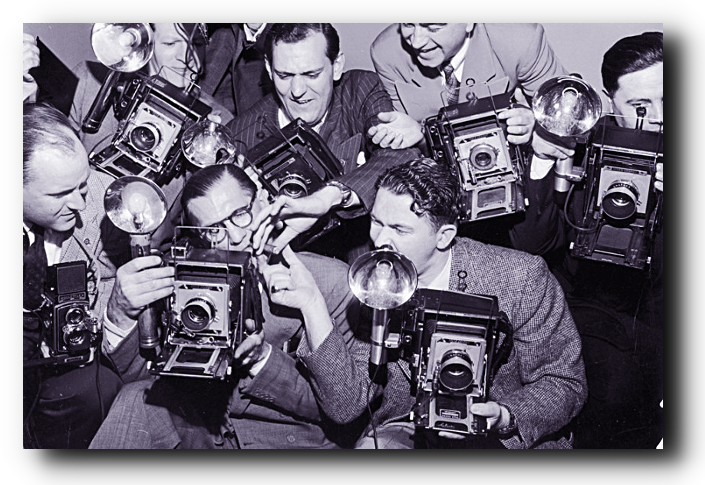
\includegraphics[angle=5,width=\linewidth]{piwigo-ajouter-photos}}%
\end{center}
  \begin{enumerate}
  \setcounter{enumi}{2}
\item Ajoutez vos photos et démarrez le transfert.

  Vos photos sont dans l'album \emph{Community}. Elles seront classées par un iconographe.
  
\end{enumerate}

  \vspace*{\fill}

  \fcolorbox{black}{white}{
  \begin{minipage}[t]{1.0\textwidth}

    \section{\faEye Soyez sélectifs}

      Nous avons déjà plus de 6000 photos, dont beaucoup se ressemblent (les
      fêtes, ça fait de chouettes photos, mais difficilement utilisables sur
      une affiche\ldots). Privilégiez donc :

      \begin{itemize}
      \item les sujets ou les traitements originaux;
      \item les gros plans;
      \item le temps couvert;
      \item le flou d'arrière-plan;
      \item les fichiers de plus de 2 Mo;
      \item les  scans d'argentique ou d'illustrations;
      \item les boîtiers \emph{reflex}.
      \end{itemize}
      
  \end{minipage}
    }
    \vspace*{\fill}
\clearpage

\section{\faTag Iconographes}

\vspace*{\fill}

\begin{enumerate}[itemsep=0mm,leftmargin=*]

\item Contactez-nous pour rejoindre l'équipe d'iconographes.
\item Affichez une photo de l'album \emph{Community}.
\item Cliquez sur \faPencil \textbf{Mots-clés}.
\item Ajoutez des mots-clés aux photos :

  \begin{itemize}
  \item Indiquez \emph{Print} si la photo convient à l'impression, \emph{Web}
    dans le cas contraire.

  \item Pour que la photo soit supprimée, indiquez \emph{Delete}.  Elle sera
    effacée plus tard
    % \footnote{1) mit Geschmacksverstärker; 2) Enthält glutenhaltige/s Getreide/-Erzeugnisse; 3) Enthält Ei/-Erzeugnisse; 4) Enthält Sojabohnen/-Erzeugnisse; 5) Enthält Sellerie/-Erzeugnisse; 6) Weizen; 7) Enthält Milch/-Erzeugnisse (laktosehaltig); 8) Enthält Sesamsamen/-Erzeugnisse; 9) Enthält Schwefeldioxid/Sulfite; 10) Enthält Erdnüsse/-Erzeugnisse; 11) Enthält Krebstiere/-Erzeugnisse; 12) Enthält Weichtiere/-Erzeugnisse; 13) Enthält Fisch/-Erzeugnisse; 14) Enthält Schalenfrüchte/Nüsse bzw. Nusserzeugnisse; 15) Gerste}.
    \footnote{mit Geschmacksverstärker;}
    \footnote{Enthält glutenhaltige/s Getreide/-Erzeugnisse;}
    \footnote{Enthält Ei/-Erzeugnisse;}
    \footnote{Enthält Sojabohnen/-Erzeugnisse;}
    \footnote{Enthält Sellerie/-Erzeugnisse;}
    \footnote{Weizen;}
    \footnote{Enthält Milch/-Erzeugnisse (laktosehaltig);}
    \footnote{Enthält Sesamsamen/-Erzeugnisse;}
    \footnote{Enthält Schwefeldioxid/Sulfite;}
    \footnote{Enthält Erdnüsse/-Erzeugnisse; }
    \footnote{Enthält Krebstiere/-Erzeugnisse;}
    \footnote{Enthält Weichtiere/-Erzeugnisse;}
    \footnote{Enthält Fisch/-Erzeugnisse;}
    \footnote{Enthält Schalenfrüchte/Nüsse bzw. Nusserzeugnisse;}
    \footnote{Gerste;}
  \end{itemize}
\end{enumerate}
  
\begin{center}
  \setlength{\fboxsep}{0pt}%
  \setlength{\fboxrule}{0pt}%
  \fbox{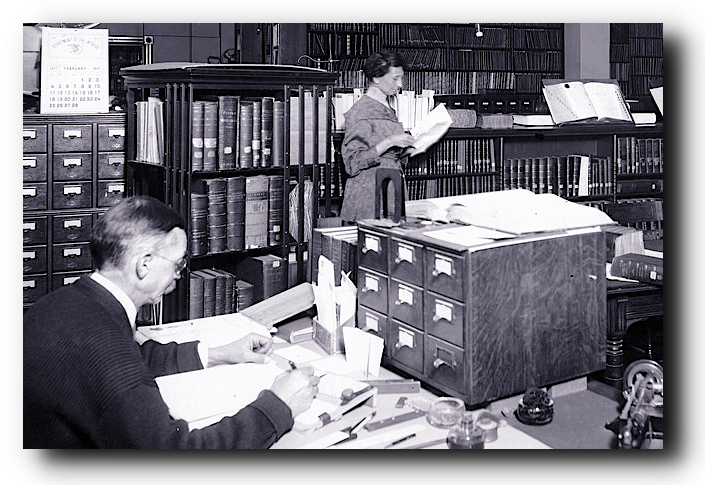
\includegraphics[angle=5,width=\linewidth]{piwigo-icono}}%
\end{center}

\vspace*{\fill}

\begin{itemize}
  \item[]
  \begin{itemize}
  \item Associez au moins les mots-clés :

    \begin{itemize}
    \item \emph{Photo} ou \emph{Illustration};
    \item \emph{Couleur} ou \emph{Monochrome};
    \item \emph{Vertical}, \emph{Carré} ou \emph{Horizontal};
    \item \emph{Intérieur} ou \emph{Extérieur};
    \item \emph{Gros plan} ou \emph{Plan large};
    \item \emph{Portrait}, \emph{Groupe}, \emph{Paysage} ou \emph{Nature morte}.
    \end{itemize}
  \end{itemize}
\end{itemize}
\vspace*{\fill}


\clearpage

\section{\faPaintBrush Graphistes}

\vspace*{\fill}

\begin{enumerate}[itemsep=0mm,leftmargin=*]

\item Cliquez sur \textbf{Mots-clés}.
\item Sélectionnez un mot-clé.
\end{enumerate}
\begin{center}
  \setlength{\fboxsep}{0pt}%
  \setlength{\fboxrule}{0pt}%
  \fbox{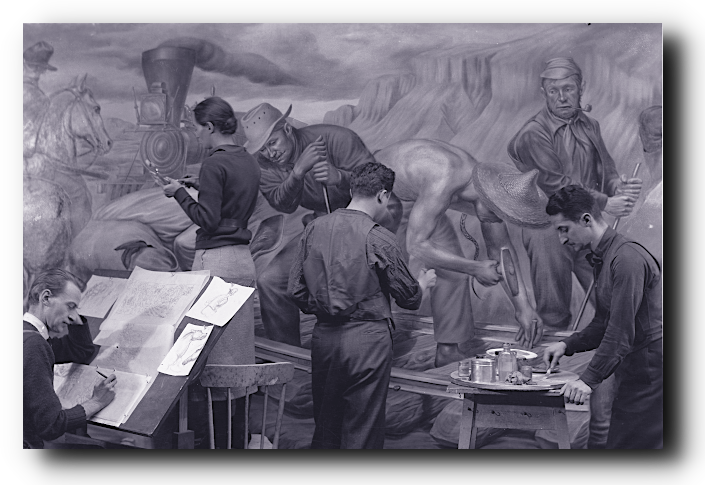
\includegraphics[angle=5,width=\linewidth]{piwigo-mots-cles-resultat}}%
\end{center}

\begin{enumerate}
  \setcounter{enumi}{2}
\item Affinez votre recherche en sélectionnant d'autres mots-clés.
\item Affichez \textbf{\textit{ze}} photo, puis téléchargez-la \faDownload.
\end{enumerate}

\vspace*{\fill}

\fcolorbox{black}{white}{
  \begin{minipage}[t]{1.0\textwidth}
\section{\faLeaf Cultiver le jardin photo}

      \emph{Le « désherbage » régulier d'un fonds est toujours
        souhaitable. Comme pour un jardin, il faut veiller à ce que la base de données
        soit toujours en bon état afin d'être efficace.}

      \emph{Il ne suffit pas d'alimenter une base; il faut s'assurer que les
        résultats qu'elle fournit sont le plus pertinents possible.  De
        nouveaux mots-clés peuvent apparaître, et il peut être plus que
        pertinent de les intégrer. Il est inutile de tout garder; il faut
        savoir trier.}

      \textsc{Profession iconographe}

      \textsc{Aurélie Lacouchie - Éditions Eyrolles}
      
  \end{minipage}
}
\vspace*{\fill}
\clearpage

\section{\faUniversity Atelier de création}

Contactez-nous pour participer à la création d'affiches en ligne
avec l'équipe \keys{\faGlobe canva.com}.

\begin{center}
  \setlength{\fboxsep}{0pt}%
  \setlength{\fboxrule}{0pt}%
  \fbox{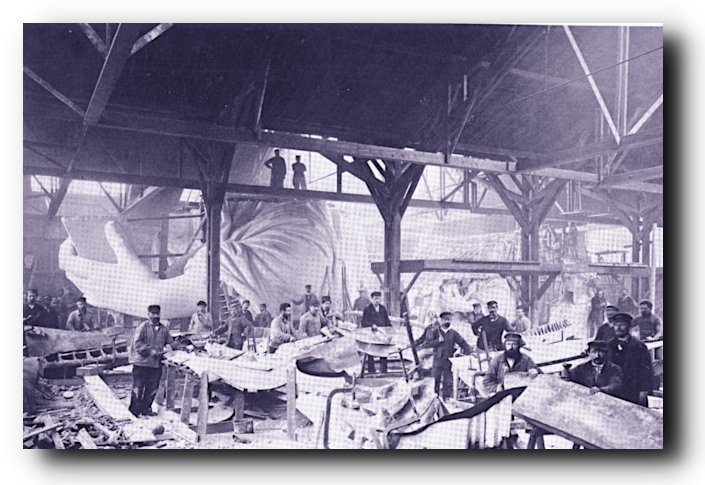
\includegraphics[angle=5,width=0.864\linewidth]{canva}}%
\end{center}
\vspace*{\fill}
\section{\faSave Sauvegarde}

Vous souhaitez protéger le patrimoine photo de l'association ?

Contactez-nous pour cloner le dépôt \emph{Git} de la galerie !
\vspace*{\fill}
\section{\faYoutube Vidéos explicatives}

\keys{\faGlobe example.com}

\begin{center}
  \setlength{\fboxsep}{0pt}%
  \setlength{\fboxrule}{0pt}%
  \fbox{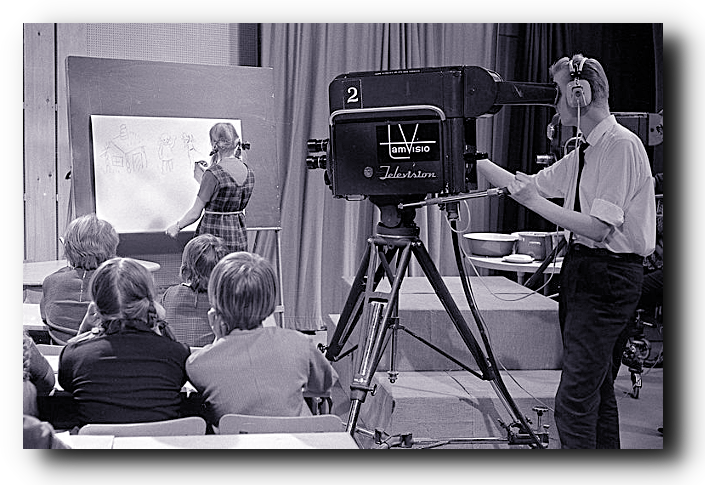
\includegraphics[angle=5,width=0.864\linewidth]{didacticiels}}%
 \end{center} 

\clearpage

\begin{center}
  \setlength{\fboxsep}{0pt}%
  \setlength{\fboxrule}{0pt}%
  \fbox{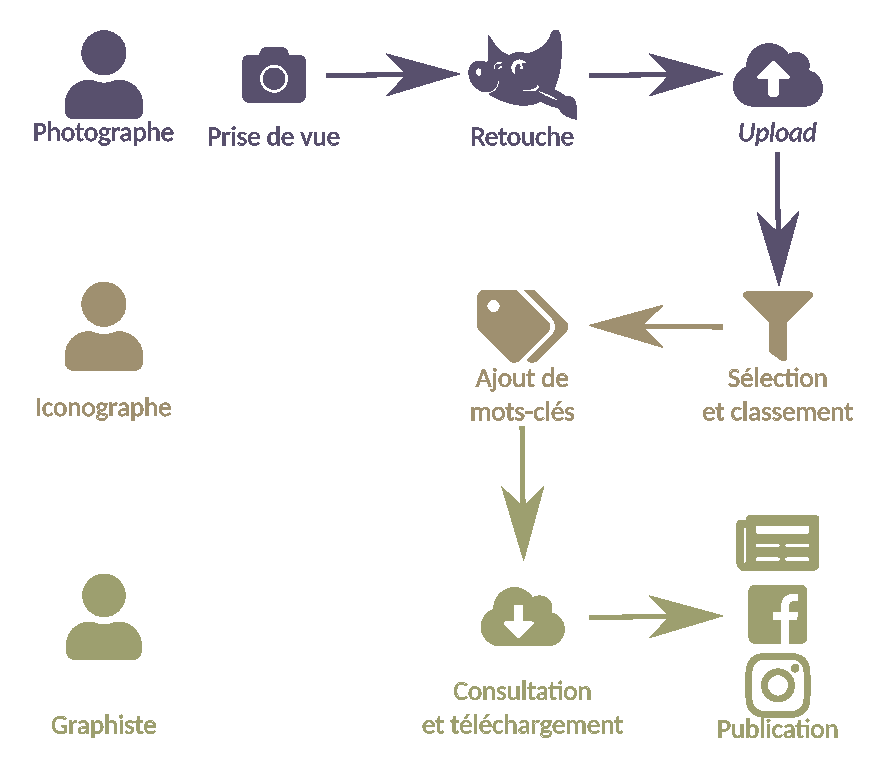
\includegraphics[angle=5,width=\linewidth]{workflow}}%

  Workflow photo
\end{center}

\vspace*{\fill}

\section{\faInfoCircle Ressources}

\begin{description}[align=right,labelwidth=4.2cm]

\item [Retouche photo] \keys{\faGlobe gimp.org/fr}

\item [Développement RAW] \keys{\faGlobe darktable.fr}

\item [PAO] \keys{\faGlobe scribus.fr}

\item [Logiciels] \keys{\faGlobe huit.re/freesoft}

\item [Photo] \keys{\faGlobe tontonphoto.fr}

\end{description}
   
\vspace*{\fill}

\section{\faEnvelope Contact}

\texttt{adress@example.com}
\vspace*{\fill}
\begin{center}
{ \textsc{Association} \\ 34,
  rue - Code postal \textsc{Ville} - Pays}

\keys{\faGlobe example.com}
\end{center}

\end{document}

